\graphicspath{{Billeder/}}
\chapter{Resultater}

\section{Resultater}
Link til Jenkins - Coverage: \url{http://ci3.ase.au.dk:8080/job/TeamTyveATMCoverage/} \newline
Som det ses på nedenstående billede virker systemet som forventet. De tracks der ligger inde i AirSpace bliver udskrevet på konsollen med alle de ønskede informationer.

De warnings der kommer, når to fly flyver for tæt, bliver udskrevet nederst i konsollen.

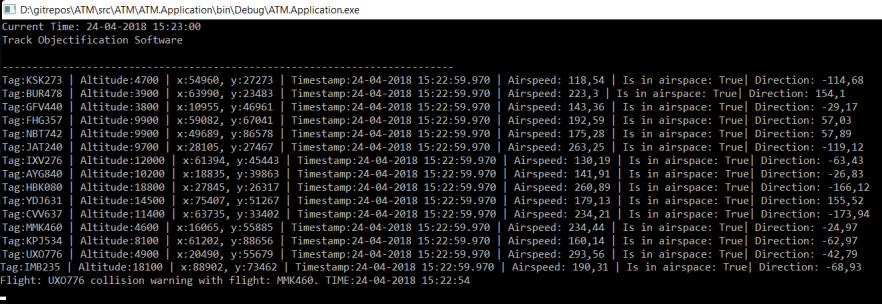
\includegraphics[scale=0.6]{1.PNG}

\section{Diskussion}
Til denne hand in var der ikke givet nogle specifikke retningslinjer for hvordan opgaven skulle løses. Dette betød også, at der var stor frihed til hvordan systemet skulle designes. \tabularnewline
Der blev valgt et design, der gjorde at Track Observation System (TOS) - klassen var meget afhængig af de andre klasser, som det også fremgår af det udarbejdede dependency tree. 
Ud fra dette, kan det også ses at det er et ret "horisontalt" system, i og med at TOS indhenter strings og objektifiserer disse. 
Når dette er gjort vil der arbejdes direkte på objekterne igennem de andre klasser, i stedet for at bruge en form for pipes and filters arkitektur, hvor der arbejdes i en vandret orden, og objekterne bearbejdes hen ad vejen i stedet for det hele på én gang. 

Dette blev i starten valgt, grundet at flere ting arbejdede på én gang. Der blev blandt andet tjekket på om flyet var i AirSpace, men også om flyet fløj for tæt på andre fly. \tabularnewline
Set i bakspejlet har det formegentlig været mere testbart at benytte en pipes and filters arkitektur, for at undgå at TOS fik så mange dependencies.

Gruppen fik dog løst det på anden måde og fik et tilfredsstillende resultat.


Der blev benyttet en CI server på Jenkins til at undersøge hvornår et build kunne merges til masteren. \tabularnewline
Dette blev dog ikke benyttet af gruppen, da det meste af systemet blev lavet da medlemmerne sad sammen fysisk på skolen.\tabularnewline
Det ville formegentlig have givet mere værdi i et større team, hvor der arbejdes mere uafhængigt af hinanden. \newline
\pagebreak
\section{Konklusion}
Alt i alt virker systemet som forventet på trods af at de måske ikke har været den optimale løsning der er blevet brugt. \tabularnewline
Set i bakspejlet kunne dette dog være løst ved at have brugt mere tid på design og arkitektur i starten af forløbet.  \tabularnewline
Gruppen har erfaret at det er vigtigt inden at der startes med implementering, at der skal laves en god arkitektur,
som også har fokus på at gøre programmet testbart. \tabularnewline
Gruppen har også erfaret at arkitekturen dermed har stor indvirkning på hvor let det er at lave integrationstest. Med en struktur hvor 
en klasse har for mange afhængigheder, som f.eks. i dette tilfælde med Track Observation System klassen, er det svært at udfører en overskuelig
intergrationstest.